\begin{figure}[h]
    \centering
    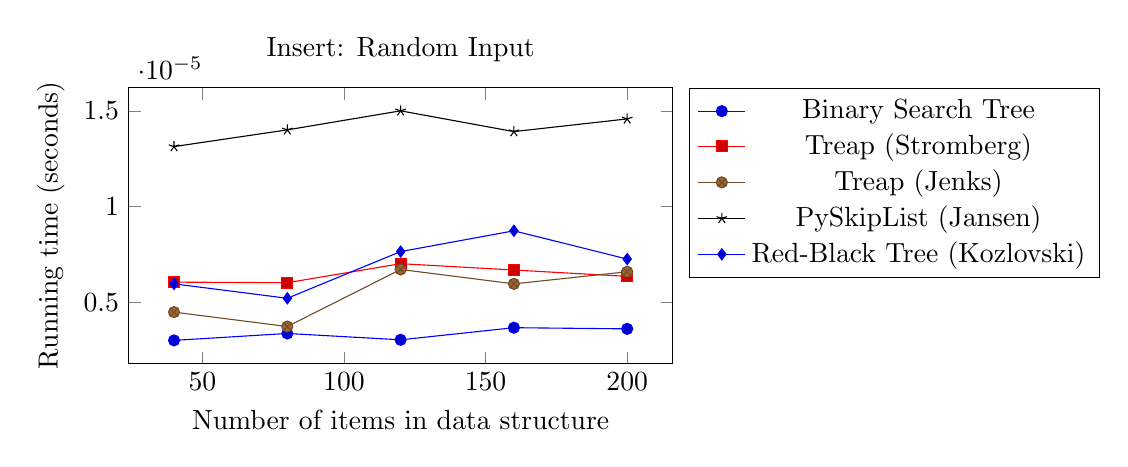
\begin{tikzpicture}
        \begin{axis}[
            xlabel={Number of items in data structure},
            ylabel={Running time (seconds)},
            title={Insert: Random Input},
            width=0.7\textwidth,
            height=2in,
            legend pos=outer north east
        ]
		\addplot coordinates {
			(40, 3.0117533675166203e-06)
			(80, 3.3731637716187535e-06)
			(120, 3.0418709011919426e-06)
			(160, 3.674339108370589e-06)
			(200, 3.6141040410199442e-06)
		};
		\addplot coordinates {
			(40, 6.053624268708563e-06)
			(80, 6.023506735033588e-06)
			(120, 7.0173853463140205e-06)
			(160, 6.686092475886862e-06)
			(200, 6.354799605460399e-06)
		};
		\addplot coordinates {
			(40, 4.487512517599434e-06)
			(80, 3.7345741757212335e-06)
			(120, 6.716210009562185e-06)
			(160, 5.963271667682596e-06)
			(200, 6.595739874861589e-06)
		};
		\addplot coordinates {
			(40, 1.3131244682372533e-05)
			(80, 1.4004653158952719e-05)
			(120, 1.4998531770233497e-05)
			(160, 1.3914300557927444e-05)
			(200, 1.4576886298781066e-05)
		};
		\addplot coordinates {
			(40, 5.96327166768329e-06)
			(80, 5.210333325803701e-06)
			(120, 7.649853553493013e-06)
			(160, 8.734084765798372e-06)
			(200, 7.258325615715211e-06)
		};
        \legend{Binary Search Tree, Treap (Stromberg), Treap (Jenks), PySkipList (Jansen), Red-Black Tree (Kozlovski)}
        \end{axis}
    \end{tikzpicture}
    \caption{Average of 10 operations, benchmarked every 40, starting at 40.}
\end{figure}